\chapter{Dây dài và sự tương ứng với hố đen}

\lectureoverview{Hố đen có entropy, nên nó phải có các bậc tự do vi mô. Ta sẽ xây dựng cách giải thích theo lý thuyết dây đơn giản nhất cho các bậc tự do ấy: trước tiên đếm các trạng thái của một dây dài bị kích thích, rồi thay đổi hằng ghép dây cho đến khi hai mô tả bằng dây và bằng hố đen gặp nhau. Đẳng thức cuối cùng được cố ý để lại như bài toán sẽ được hoàn tất ở buổi giảng sau.}

\section{Entropy đòi hỏi các vật mang ở cấp vi mô}

Nói rằng một hệ có entropy lớn tức là nói rằng nó có thể che giấu một lượng lớn thông tin vi mô. Một bồn tắm nước nóng có thể có entropy cỡ \(10^{30}\). Chỉ riêng phát biểu đó đã cho ta biết rằng có cực kỳ nhiều bậc tự do vi mô, bất kể ta có chọn khảo sát chúng từng phân tử một hay không. Nhiệt động lực học có thể xác định entropy bằng cách đo năng lượng và nhiệt độ, nhưng nó không nhận diện các đối tượng mang nó.

Động lực học chất lưu làm cho sự phân biệt này trở nên quen thuộc. Nó mô tả mật độ, vận tốc, áp suất và dòng chảy vĩ mô mà không nhắc đến nguyên tử. Thêm nhiệt động lực học vào, ta phát hiện rằng chất lưu có entropy. Entropy báo hiệu một cấu trúc vi mô mà các phương trình thô hạt không hiển lộ; nó gợi ra một câu hỏi mới chứ không trả lời câu hỏi đó.

Hố đen đặt ra cùng một thách thức, nhưng ở dạng sắc nét hơn. Đề xuất của Bekenstein, được hoàn tất bởi phép tính của Hawking, gán cho nó một entropy tỉ lệ với diện tích chân trời. Thuyết tương đối rộng xác định hình học và nhiệt động lực học của nó, nhưng không cho bản kiểm kê nào về các trạng thái vi mô. Đâu là những đối tượng nhỏ bé và đông đảo mà các cấu hình của chúng giải thích được định luật diện tích? Trong lý thuyết dây có một ứng viên cụ thể. Lập luận được phát triển ở đây có chủ ý là định tính: nó cho đúng sự phụ thuộc tham số, đồng thời lược bỏ các hằng số số học và bộ máy hình thức của một phép đếm trạng thái đầy đủ.

\section{Ba thang đo và một điểm dễ nhầm về ký hiệu}

Hấp dẫn cung cấp một độ dài đặc biệt, độ dài Planck,
\begin{equation}
\ell_p=\sqrt{\frac{G_N\hbar}{c^3}}.
\label{eq:l06-planck-si}
\end{equation}

\begin{classroomqa}
\audiencequestion{Tổ hợp nào của \(G_N\), \(\hbar\) và \(c\) cho ra độ dài Planck?\lecturetimestamp{00:06:08}}
\lecturerresponse{Đó là \(\sqrt{G_N\hbar/c^3}\), khoảng \(10^{-33}\) centimét. Ta sẽ lập tức đặt \(\hbar=c=1\), nên hệ thức trở nên đơn giản hơn nhiều.}
\end{classroomqa}

Trong đơn vị tự nhiên,
\begin{equation}
\hbar=c=1,
\qquad
G_N=\ell_p^2.
\label{eq:l06-planck-area}
\end{equation}
Vì thế hằng số Newton có thứ nguyên của diện tích. Bởi vậy, một diện tích chia cho \(G_N\) là vô thứ nguyên và có thể là entropy.

Lý thuyết dây có một độ dài thứ hai, \(\ell_s\). Khi đun nóng một dây, hoặc đặt nó vào trạng thái kích thích mạnh, nó ngoằn ngoèo trên nhiều thang độ dài. Thang ngắn nhất đặc trưng trong bức tranh sơ cấp này là độ dài dây. Có thể xem \(\ell_s\) là kích thước gắn với một đơn vị cơ bản của dao động dây.

Đại lượng thứ ba là hằng ghép dây vô thứ nguyên \(g_s\). Nó chi phối sự tách và nhập: một dây có thể thắt lại thành hai dây, hoặc một dây kích thích có thể phát ra một lượng tử dây kín.

\begin{classroomqa}
\audiencequestion{Ý nghĩa vật lý của hằng ghép dây là gì?\lecturetimestamp{00:09:20}}
\lecturerresponse{Nó chi phối khả năng xảy ra một tương tác của dây, chẳng hạn sự tách khi một dây tự giao với chính nó. Chính xác hơn, \(g_s\) là biên độ tương tác; một xác suất hay tốc độ tương ứng bắt đầu ở bậc \(g_s^2\).}
\end{classroomqa}

Kích thích dây kín không khối lượng được phát ra có thể là một graviton. Theo nghĩa đó \(g_s\) đóng vai trò tương tự điện tích: nó là hệ số gắn với một đỉnh tương tác.\editorialnote{Trong bài giảng, \(g_s\) lúc được gọi là xác suất, lúc là biên độ. Trong lý thuyết nhiễu loạn, nó là hằng ghép ở mức biên độ; xác suất và tốc độ chứa bình phương của nó.}

\section{Vì sao hấp dẫn phụ thuộc vào \texorpdfstring{\(g_s^2\)}{bình phương của hằng ghép}}

Trước hết hãy xét bức tranh trao đổi trong điện từ học. Một vật mang điện phát ra một photon với hệ số \(e\), và một vật thứ hai hấp thụ nó với thêm một hệ số \(e\). Vì vậy biên độ trao đổi chứa \(e^2\). Bức tranh này không phải là câu chuyện theo nghĩa đen về một vật phóng cổ điển, nhưng nó cho thấy đúng cách hằng ghép đi vào.

\begin{figure}[htbp]
\centering
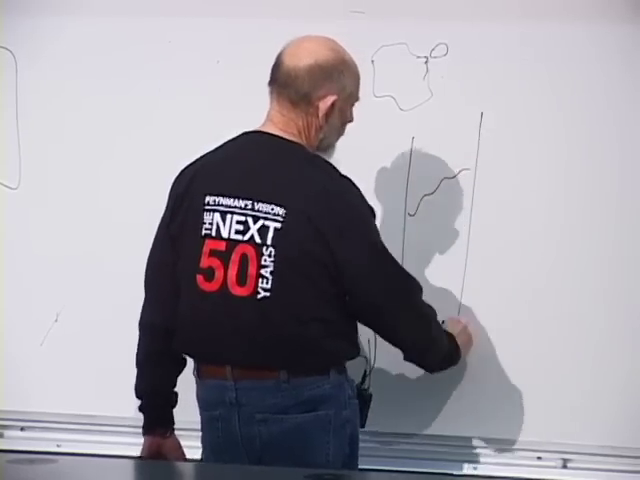
\includegraphics[width=0.72\textwidth]{lecture_06_figure_03.png}
\caption{Các phác họa hoàn chỉnh về quá trình trao đổi trên bảng: một hằng ghép gắn tại điểm phát và lại gắn thêm một lần nữa tại điểm hấp thụ.}
\lectureframe{00:11:30.000}
\end{figure}

Trong phiên bản của lý thuyết dây, photon được thay bằng graviton và điện tích được thay bằng \(g_s\). Một hệ số đi kèm sự phát ra và một hệ số khác đi kèm sự hấp thụ, nên độ mạnh hấp dẫn tỉ lệ như \(g_s^2\).

Ở khoảng cách lớn, chính tương tác ấy phải tái tạo định luật lực Newton,
\begin{equation}
F_{\mathrm{grav}}\sim G_N\frac{M_1M_2}{r^2}.
\end{equation}
Các khối lượng và sự phụ thuộc nghịch đảo bình phương mô tả nguồn và sự lan truyền; điều cần ở đây là hằng ghép nhân với chúng.

\begin{figure}[htbp]
\centering
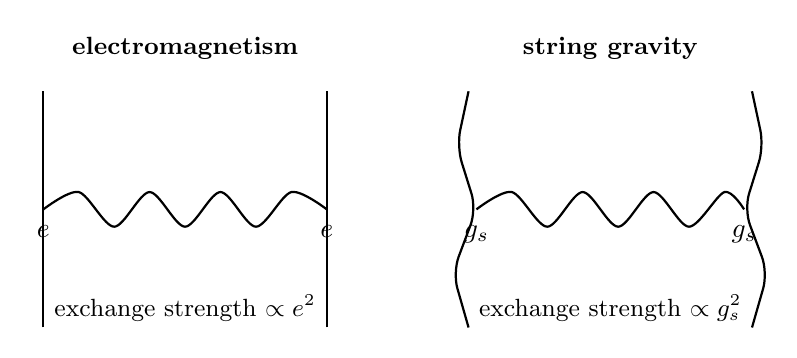
\begin{tikzpicture}[x=1cm,y=1cm]
  \node[font=\small\bfseries] at (1.8,3.55) {electromagnetism};
  \draw[line width=0.8pt] (0,0) -- (0,3);
  \draw[line width=0.8pt] (3.6,0) -- (3.6,3);
  \draw[line width=0.8pt] plot[smooth] coordinates {(0,1.5) (0.45,1.72) (0.9,1.28) (1.35,1.72) (1.8,1.28) (2.25,1.72) (2.7,1.28) (3.15,1.72) (3.6,1.5)};
  \node[below] at (0,1.42) {\(e\)};
  \node[below] at (3.6,1.42) {\(e\)};
  \node[font=\small] at (1.8,0.25) {exchange strength \(\propto e^2\)};
  \node[font=\small\bfseries] at (7.2,3.55) {string gravity};
  \draw[line width=0.8pt,rounded corners=6pt] (5.4,0) -- (5.2,0.7) -- (5.5,1.5) -- (5.25,2.3) -- (5.4,3);
  \draw[line width=0.8pt,rounded corners=6pt] (9,0) -- (9.2,0.7) -- (8.9,1.5) -- (9.15,2.3) -- (9,3);
  \draw[line width=0.8pt] plot[smooth] coordinates {(5.5,1.5) (5.95,1.72) (6.4,1.28) (6.85,1.72) (7.3,1.28) (7.75,1.72) (8.2,1.28) (8.65,1.72) (8.9,1.5)};
  \node[below] at (5.5,1.42) {\(g_s\)};
  \node[below] at (8.9,1.42) {\(g_s\)};
  \node[font=\small] at (7.2,0.25) {exchange strength \(\propto g_s^2\)};
\end{tikzpicture}
\caption{Phép tương tự bằng cách đếm hằng ghép. Mỗi đầu của lượng tử được trao đổi đóng góp một hệ số tương tác.}
\end{figure}

Nhận xét này gần như xác định hằng số Newton. Hằng ghép \(g_s\) là vô thứ nguyên, còn trong bốn chiều \(G_N\) có thứ nguyên là độ dài bình phương. Độ dài vi mô sẵn có là \(\ell_s\), do đó
\begin{equation}
G_N\sim g_s^2\ell_s^2.
\label{eq:l06-newton-string}
\end{equation}
Kết hợp điều này với Phương trình~\eqref{eq:l06-planck-area} ta được
\begin{equation}
\ell_p\sim g_s\ell_s.
\label{eq:l06-planck-string}
\end{equation}

\begin{figure}[htbp]
\centering
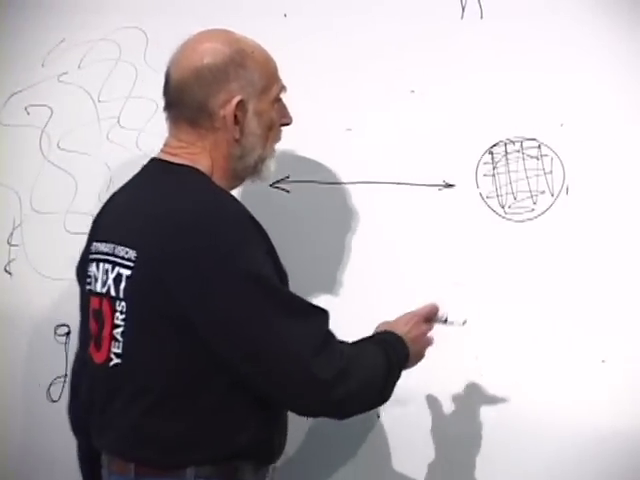
\includegraphics[width=0.72\textwidth]{lecture_06_figure_04.png}
\caption{Các hệ thức cơ bản được giữ lại trên bảng: \(\ell_p^2=G_N\) và \(\ell_p\sim g_s\ell_s\).}
\lectureframe{00:15:45.000}
\end{figure}

Phương trình~\eqref{eq:l06-newton-string} là hệ thức rút gọn được dùng xuyên suốt bài giảng này.\editorialnote{Trong lý thuyết dây đã compact hóa, hằng số Newton hiệu dụng bốn chiều còn phụ thuộc vào thể tích compact hóa và các quy ước hệ số cỡ một. Bài giảng lược bỏ những dữ liệu ấy để tách riêng luật tỉ lệ của phép tương ứng.}

\begin{classroomqa}
\audiencequestion{\(g_s\) lớn hơn hay nhỏ hơn một, và độ dài nào lớn hơn?\lecturetimestamp{00:16:00}}
\lecturerresponse{Ta làm việc ở ghép yếu, \(g_s<1\). Khi đó \(\ell_p\sim g_s\ell_s\) suy ra rằng độ dài dây lớn hơn độ dài Planck. Ghép mạnh đòi hỏi một mô tả khác và không cần ở đây.}
\end{classroomqa}

\section{Phép đếm cho hố đen}

Bỏ qua hằng số Boltzmann và các hệ số số học, entropy Bekenstein--Hawking là
\begin{equation}
S_{\mathrm{BH}}=\frac{A}{4G_N}sim\frac{A}{G_N}sim\frac{A}{\ell_p^2}.
\label{eq:l06-bh-area}
\end{equation}
Hệ số \(1/4\) là chính xác trong công thức bán cổ điển, nhưng nó sẽ không đóng vai trò nào trong lập luận theo luật tỉ lệ này.

\begin{classroomqa}
\audiencequestion{Chỉ số dưới ``BH'' có nghĩa là black hole hay Bekenstein--Hawking?\lecturetimestamp{00:16:51}}
\lecturerresponse{Với mục đích của ta, nó có thể gợi nhắc cả hai. Điều quan trọng là entropy bằng diện tích chân trời được đo theo các diện tích Planck.}
\end{classroomqa}

Đối với một hố đen Schwarzschild bốn chiều,
\begin{equation}
R_s=2G_NM,
\qquad
A=4\pi R_s^2.
\end{equation}
Bỏ qua \(2\) và \(4\pi\) như trong bài giảng,
\begin{align}
S_{\mathrm{BH}}
&\sim \frac{R_s^2}{G_N}
\sim \frac{(G_NM)^2}{G_N} \\
&\sim M^2G_N
\sim M^2\ell_p^2.
\label{eq:l06-bh-mass}
\end{align}
Đây là dạng ta sẽ so sánh với phép đếm của dây.

\section{Một dây dài như một bước đi ngẫu nhiên}

Hãy bắt đầu với một dây nhỏ và bơm năng lượng vào nó. Một dây kích thích mạnh điển hình không còn là một vòng gọn gàng. Nó trở thành một vật thể dài, rối mù, như dây câu sau khi ống cuộn bị rối tung. Mớ rối ấy có entropy vì một số lượng khổng lồ cấu hình trông giống nhau ở mức vĩ mô.

Để đếm chúng, hãy thay không gian bằng một mạng mà các link có độ dài \(\ell_s\). Các site là các đỉnh, các link là các đoạn thẳng, và các ô vuông cơ bản là các plaquette. Một dây được biểu diễn bằng một dãy liên thông các link. Mô hình này có chủ ý là thô sơ, nhưng phép đếm trạng thái tăng theo hàm mũ của nó nắm bắt được luật tỉ lệ mong muốn.

\begin{figure}[htbp]
\centering
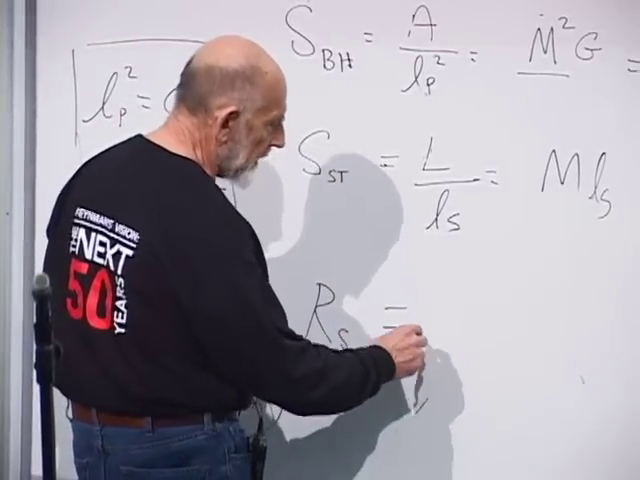
\includegraphics[width=0.72\textwidth]{lecture_06_figure_05.png}
\caption{Mô hình mạng hai chiều. Đoạn màu xanh đánh dấu một bước của dây; bốn khả năng tiếp diễn được đếm tại mỗi site.}
\lectureframe{00:23:50.000}
\end{figure}

\begin{classroomqa}
\audiencequestion{Có bao nhiêu lựa chọn ở mỗi bước của bước đi mô hình?\lecturetimestamp{00:22:43}}
\lecturerresponse{Là bốn trên mạng vuông, vì cho phép quay lui ngay lập tức. Trong ba chiều sẽ là sáu. Một mạng khác sẽ thay đổi con số thông thường, nhưng không thay đổi sự thật rằng số bước đi tăng theo hàm mũ với số link.}
\end{classroomqa}

Nếu dây có \(n\) link, thì phép đếm mô hình hai chiều là
\begin{equation}
\Omega_n\sim4^n.
\label{eq:l06-walk-count}
\end{equation}
Có một bước đi thẳng ngoại lệ, nhưng đó chỉ là một trạng thái trong \(4^n\). Một bước đi điển hình gấp khúc lặp đi lặp lại và chiếm một khối cầu rối. Với \(n\) lớn, hầu như mọi cấu hình được sinh ngẫu nhiên đều giống nhau về mặt định tính.

Entropy là logarit của số cấu hình không thể phân biệt ở mức vĩ mô:
\begin{equation}
S_{\mathrm{st}}=\log\Omega_n\sim n\log4\sim n.
\label{eq:l06-string-entropy-n}
\end{equation}

\begin{classroomqa}
\audiencequestion{Vì sao entropy lại tỉ lệ với \(n\) chứ không phải với \(4^n\)?\lecturetimestamp{00:25:39}}
\lecturerresponse{Entropy là logarit của số trạng thái. Do đó \(\log(4^n)=n\log4\), còn hệ số \(\log4\) là một hằng số cỡ một mà ta sẽ lược bỏ.}
\end{classroomqa}

Nếu \(L\) là độ dài đường cong thu được khi đi dọc theo dây từ đầu này đến đầu kia, thì
\begin{equation}
n=\frac{L}{\ell_s},
\qquad
S_{\mathrm{st}}\sim\frac{L}{\ell_s}.
\label{eq:l06-string-entropy-length}
\end{equation}
Ở đây \(L\) không phải là đường kính của khối rối. Nó là quãng đường dài hơn nhiều được đo dọc theo dây.

Tiếp theo ta đổi từ độ dài đường cong sang khối lượng. Với \(c=\hbar=1\), khối lượng có thứ nguyên là nghịch đảo của độ dài. Vì vậy một link cỡ dây mang khối lượng cỡ
\begin{equation}
m_{\mathrm{link}}\sim\frac{1}{\ell_s}.
\label{eq:l06-link-mass}
\end{equation}

\begin{classroomqa}
\audiencequestion{Vì sao khối lượng của một link phải tỉ lệ như \(1/\ell_s\)?\lecturetimestamp{00:29:20}}
\lecturerresponse{Trong các đơn vị này, khối lượng là nghịch đảo của độ dài, và \(\ell_s\) là độ dài sẵn có duy nhất. Tương đương, sức căng dây cỡ \(1/\ell_s^2\) nhân với độ dài link \(\ell_s\) cho cùng kết quả.}
\end{classroomqa}

Khi đó toàn bộ dây có
\begin{equation}
M\sim n m_{\mathrm{link}}
\sim\frac{n}{\ell_s}
\sim\frac{L}{\ell_s^2},
\qquad
L\sim M\ell_s^2.
\label{eq:l06-string-mass}
\end{equation}
Thế vào Phương trình~\eqref{eq:l06-string-entropy-length} ta được
\begin{equation}
S_{\mathrm{st}}\sim M\ell_s.
\label{eq:l06-string-entropy-mass}
\end{equation}
Bước đi trên mạng bỏ qua các ràng buộc của mặt thế giới và các hệ số số học, nhưng sự tăng theo hàm mũ của phổ dây kích thích mạnh cho cùng luật tỉ lệ dẫn đầu này.\editorialnote{Cấu trúc bước đi ngẫu nhiên là một mẹo ghi nhớ cho mật độ trạng thái của dây ở mức kích thích cao, chứ không phải một phép rời rạc hóa theo nghĩa đen của một dây cơ bản.}

\section{Sự không khớp mở đầu cho lập luận}

Giờ đây hai kết quả là
\begin{equation}
S_{\mathrm{BH}}\sim M^2\ell_p^2,
\qquad
S_{\mathrm{st}}\sim M\ell_s.
\label{eq:l06-two-entropies}
\end{equation}
Chúng giống nhau, nhưng không bằng nhau khi khối lượng cố định và hằng ghép tùy ý. Biểu thức của hố đen là bậc hai theo \(M\); biểu thức của dây là tuyến tính. Không thể đơn giản tuyên bố một dây nóng là hố đen mà không giải thích hai miền đó gặp nhau như thế nào.

\begin{figure}[htbp]
\centering
\includegraphics[width=0.78\textwidth]{lecture_06_figure_06.png}
\caption{Phép so sánh trên bảng không bị che khuất: entropy hố đen ở trên, entropy dây dài ở dưới, với các hệ thức Planck--dây được giữ lại ở bên trái.}
\lectureframe{00:33:20.000}
\end{figure}

Đây là chỗ lớp học tạm dừng. Sự hồi hộp này có ích: sự không khớp không phải là thất bại của ý tưởng, mà là manh mối cho thấy phải so sánh cùng một trạng thái trong khi thay đổi độ mạnh của hấp dẫn.

\section{Xoay núm điều chỉnh hằng ghép}

Giữ \(\ell_s\) cố định và hình dung rằng \(g_s\) có thể thay đổi. Tại \(g_s=0\), dây không tách cũng không nhập và hấp dẫn biến mất vì \(G_N\sim g_s^2\ell_s^2\). Khi đó một trạng thái có năng lượng đủ lớn là một dây dài tương tác yếu.

Tăng \(g_s\) từ từ. Các tương tác của dây trở nên khả dĩ và, quan trọng hơn đối với lập luận hiện tại, hấp dẫn mạnh lên.

\begin{classroomqa}
\audiencequestion{Khi \(g_s\) tăng, liệu hiệu ứng đầu tiên có đơn giản chỉ là dây tách thành những dây ngắn hơn không?\lecturetimestamp{00:36:29}}
\lecturerresponse{Sự tách và nhập trở nên khả dĩ, nhưng hãy giữ \(\ell_s\) cố định và theo dõi trạng thái entropy cao. Hiệu ứng trung tâm là \(G_N\) tăng lên, nên tự hấp dẫn của dây dài kéo khối rối co vào trong.}
\end{classroomqa}

Vật thể co lại và trở nên đậm đặc hơn. Thế năng hấp dẫn của nó là âm, nên sự co lại làm giảm tổng năng lượng của nó và do đó làm giảm khối lượng.

\begin{classroomqa}
\audiencequestion{Năng lượng tăng hay giảm khi tự hấp dẫn kéo dây lại với nhau?\lecturetimestamp{00:37:48}}
\lecturerresponse{Nó giảm. Năng lượng liên kết trở nên âm hơn. Khối lượng dọc theo quá trình đó không nhất thiết phải giữ cố định dù ta vẫn tiếp tục theo dõi cùng một trạng thái.}
\end{classroomqa}

Cuối cùng, kích thước của vật trở nên cùng bậc với bán kính Schwarzschild của nó. Vượt quá điểm đó, mô tả lỗ đen là cách mô tả tự nhiên. Một kích thích ban đầu lớn hơn đạt tới điều kiện này ở hằng số liên kết nhỏ hơn, vì một vật có khối lượng lớn hơn cần độ mạnh hấp dẫn nhỏ hơn để hình thành chân trời.

\begin{figure}[htbp]
\centering
\resizebox{0.95\linewidth}{!}{%
\begin{tikzpicture}[x=1cm,y=1cm,>=Latex]
  \draw[->,line width=0.9pt] (0,0) -- (11,0) node[right] {increasing \(g_s\)};
  \node[draw,rounded corners,align=center,minimum width=2.6cm,minimum height=1.15cm] at (1.8,1.5) {long excited string\\weak self-gravity};
  \node[draw,rounded corners,align=center,minimum width=2.6cm,minimum height=1.15cm] at (5.5,1.5) {correspondence point\\\(R_s\sim\ell_s\)};
  \node[draw,circle,align=center,minimum size=1.8cm] at (9.3,1.5) {black\\hole};
  \draw[->,line width=0.8pt] (3.15,1.5) -- (4.1,1.5) node[midway,above,font=\small] {contracts};
  \draw[->,line width=0.8pt] (6.9,1.5) -- (8.25,1.5);
  \node[font=\small,align=center] at (5.5,-0.65) {same family of states followed slowly;\\binding energy and mass may change};
\end{tikzpicture}
}
\caption{Quỹ đạo tương ứng khi giữ \(\ell_s\) cố định. Đảo ngược mũi tên đưa trạng thái lỗ đen trở lại trạng thái dây dài.}
\end{figure}

\begin{classroomqa}
\audiencequestion{Ta có nên hình dung \(g_s\) nằm giữa 0 và 1 không?\lecturetimestamp{00:40:18}}
\lecturerresponse{Có. Lập luận vẫn nằm trong miền liên kết yếu. Nếu \(g_s\) rất nhỏ, thì trạng thái đó phải có khối lượng lớn tương ứng trước khi trở thành lỗ đen. Chúng ta không cần đi vào miền \(g_s>1\) được kiểm soát kém.}
\end{classroomqa}

Sự thay đổi chậm là thuận nghịch trong thí nghiệm tưởng tượng này.

\begin{classroomqa}
\audiencequestion{Nếu ta hạ hằng số liên kết trở lại cho đến khi hấp dẫn không còn có thể giữ lỗ đen gắn kết nữa, thì nó trở thành gì?\lecturetimestamp{00:41:37}}
\lecturerresponse{Một dây dài. Khi hấp dẫn triệt tiêu, mọi thứ trong cách xây dựng này đều phải được mô tả bằng các trạng thái dây. Xoay núm điều chỉnh theo một chiều sẽ ánh xạ dây thành lỗ đen; xoay ngược lại sẽ ánh xạ lỗ đen thành dây.}
\end{classroomqa}

Với tổng năng lượng cố định và trong một thể tích cố định, cấu hình entropy cao chiếm ưu thế về cơ bản là một dây dài chứ không phải một số lượng khổng lồ các dây ngắn. Mệnh đề đó không được suy ra ở đây. Đó là kết quả của cơ học thống kê của các dây gần chế độ Hagedorn và sẽ được quay lại sau.

\section{Những gì người quan sát bên ngoài thấy}

Dây ở đâu khi vật được mô tả là một lỗ đen? Trong mô tả từ bên ngoài, nó không đột ngột biến mất. Thời gian Schwarzschild đẩy sự băng qua biểu kiến tới thời điểm muộn tùy ý, nên các bậc tự do dạng dây được biểu diễn như đang tích tụ trên hoặc gần chân trời.

\begin{figure}[htbp]
\centering
\includegraphics[width=0.72\textwidth]{lecture_06_figure_07.png}
\caption{So sánh trên bảng giữa một chân trời vĩ mô, nơi cấu trúc ở thang dây chỉ là một lớp mờ mỏng, và một chân trời nhỏ hơn có bán kính tiến gần tới thang kích thước vòng.}
\lectureframe{00:45:30.000}
\end{figure}

Khi \(R_s\gg\ell_s\), lỗ đen là vĩ mô và cấu trúc ở thang dây chỉ là một lớp mỏng so với bán kính chân trời. Khi bán kính giảm xuống gần \(\ell_s\), sự phân biệt giữa một lỗ đen trơn và một dây mở rộng mất đi ý nghĩa. Đây là mô tả bên ngoài theo chân trời kéo giãn; không nên nhầm nó với một khẳng định độc lập với tọa độ rằng vật chất rơi vào không bao giờ đi qua một chân trời chính quy.\editorialnote{Bài giảng dùng mô tả bên ngoài quen thuộc trong nguyên lý bổ sung lỗ đen. Cụm ``trên chân trời'' chỉ các bậc tự do được phân giải trong mô tả từ bên ngoài, chứ không phải một suy dẫn riêng về vị trí hiệp biến của chúng.}

Sự chuyển tiếp xảy ra khi
\begin{equation}
R_s\sim\ell_s.
\label{eq:l06-correspondence-radius}
\end{equation}
Bên dưới thang dây, hình học Schwarzschild không thể phân giải cấu trúc được cho là nâng đỡ nó. Các vòng dao động rời khỏi chân trời lẽ ra sẽ có, và trạng thái ấy đúng hơn nên được gọi là một dây.

\section{Điểm tương ứng}

Dùng \(R_s\sim G_NM\) trong Phương trình~\eqref{eq:l06-correspondence-radius}:
\begin{equation}
G_NM\sim\ell_s.
\end{equation}
Sau đó thế \(G_N\sim g_s^2\ell_s^2\):
\begin{equation}
M g_s^2\ell_s^2\sim\ell_s,
\qquad
M g_s^2\ell_s\sim1.
\label{eq:l06-correspondence-condition}
\end{equation}

\begin{figure}[htbp]
\centering
\includegraphics[width=0.72\textwidth]{lecture_06_figure_08.png}
\caption{Phần đại số hoàn chỉnh của sự chuyển tiếp trên bảng: \(R_s\sim\ell_s\) dẫn tới điều kiện vô thứ nguyên được đóng khung \(Mg_s^2\ell_s\sim1\).}
\lectureframe{00:49:50.000}
\end{figure}

Một người nghe nhận ra điều kiện này đang chuẩn bị cho điều gì. Tại điểm tương ứng,
\begin{align}
S_{\mathrm{BH}}
&\sim M^2\ell_p^2
\sim M^2g_s^2\ell_s^2 \\
&=(M\ell_s)(Mg_s^2\ell_s)
\sim M\ell_s
\sim S_{\mathrm{st}}.
\label{eq:l06-entropy-preview}
\end{align}

\begin{classroomqa}
\audiencequestion{Các phương trình đã ngụ ý rằng entropy của lỗ đen và của dây trở nên bằng nhau hay chưa?\lecturetimestamp{00:50:18}}
\lecturerresponse{Đúng. Đó chính là hướng mà phép tính đang đi tới. Các thành phần đã được đặt lên bảng, nhưng bài giảng hoãn việc lắp ghép đầy đủ chúng lại để có thể xem xét cẩn thận logic của phép tương ứng.}
\end{classroomqa}

Phương trình~\eqref{eq:l06-entropy-preview} là bản xem trước đại số một dòng hàm ẩn trong phần trao đổi đó. Nó xác lập quy luật tỉ lệ, không phải hệ số chính xác \(1/4\). Những sự khớp vi mô chính xác đòi hỏi các lỗ đen được kiểm soát tốt hơn và các cấu trúc dây chi tiết hơn.\editorialnote{Bài giảng dừng lại trước khi trình bày Phương trình~\eqref{eq:l06-entropy-preview} như một phép suy dẫn hoàn chỉnh. Nó được viết ra ở đây vì người nghe đã nêu đích danh sự bằng nhau ấy và mọi hệ thức cần thiết đều đã xuất hiện.}

\section{Vì sao entropy có thể được chuyển qua}

Còn lại một thành phần logic nữa. Giả sử một tham số điều khiển, chẳng hạn như từ trường hay \(g_s\), được biến thiên đủ chậm trong khi hệ được cô lập và tiến hóa là thuận nghịch. Năng lượng, kích thước và mức độ liên kết có thể thay đổi, nhưng entropy được bảo toàn:
\begin{equation}
\Delta S=0.
\label{eq:l06-adiabatic-entropy}
\end{equation}
Bài giảng nối điều này với sự bảo toàn thông tin. Entropy đo lượng thông tin bị che khuất bởi một mô tả thô hoá; một sự thay đổi chậm, thuận nghịch của Hamiltonian sắp xếp lại các trạng thái mà không xóa đi thông tin đó.

\begin{classroomqa}
\audiencequestion{Entropy không đổi có đòi hỏi rằng đường đi phải tránh một chuyển pha không?\lecturetimestamp{00:54:01}}
\lecturerresponse{Có, phải có thể theo dõi trạng thái một cách liên tục. Một hệ hữu hạn không có chuyển pha nhiệt động học phi giải tích đúng nghĩa kiểu thể tích vô hạn, và nếu sự thay đổi đủ chậm thì phép tương ứng có thể được xem như một sự chuyển tiếp trơn.}
\end{classroomqa}

Ở đây, đoạn nhiệt được dùng theo nghĩa mạnh hơn, gần tĩnh và thuận nghịch. Một quá trình đoạn nhiệt nhưng không thuận nghịch có thể sinh entropy; sự chậm và khả năng theo dõi trạng thái là thiết yếu.\editorialnote{Mệnh đề nhiệt động học \(\Delta S=0\) đòi hỏi một đường đi đoạn nhiệt thuận nghịch. Về mặt cơ học lượng tử, ý tưởng tương ứng là bám theo cùng một tập trạng thái khi một tham số thay đổi mà không có các chuyển mức mất kiểm soát.}

\begin{classroomqa}
\audiencequestion{Vì sao một dây dài lại có entropy lớn hơn vài dây ngắn hơn mang cùng tổng khối lượng?\lecturetimestamp{00:54:44}}
\lecturerresponse{Điều đó trái trực giác, nhưng phép đếm tường minh các trạng thái năng lượng cao ưu ái một thành phần dây dài trong một thể tích cố định. Chứng minh được để lại sau; đối với lập luận hiện tại, ta chỉ cần rằng lỗ đen được ánh xạ vào sector dây entropy cực đại, chứ không phải vào một khí loãng gồm rất nhiều dây ngắn.}
\end{classroomqa}

Vì vậy, chiến lược thực hiện là:
\begin{enumerate}
\item Bắt đầu với một lỗ đen khối lượng \(M_0\) ở hằng số liên kết \(g_{s,0}\).
\item Giảm \(g_s\) từ từ trong khi bám theo cùng một họ trạng thái entropy cao.
\item Dừng ở \(R_s\sim\ell_s\), nơi mô tả lỗ đen chuyển thành mô tả dây dài.
\item Đếm các trạng thái dây bằng \(S_{\mathrm{st}}\sim M\ell_s\).
\item Mang entropy đó trở lại dọc theo đường đi thuận nghịch tới lỗ đen ban đầu.
\end{enumerate}

\begin{figure}[htbp]
\centering
\includegraphics[width=0.72\textwidth]{lecture_06_figure_09.png}
\caption{Nguyên lý được giữ lại trên bảng trong khi trình bày chiến lược: một sự thay đổi đoạn nhiệt của \(g_s\) không làm thay đổi \(S\).}
\lectureframe{00:56:40.000}
\end{figure}

Lý thuyết dây đã cho ra những phép đếm entropy sắc nét hơn nhiều cho các lỗ đen mang điện, quay, siêu đối xứng, gần cực trị và ở số chiều cao hơn. Thảo luận về Schwarzschild trung hòa ở đây là lập luận tương ứng gần đúng: nó xác định sự phụ thuộc theo tham số của mật độ trạng thái và sự chuyển tiếp vật lý, chứ không phải một độ suy biến được bảo vệ một cách chính xác.\editorialnote{Sự phù hợp chính xác là mạnh nhất đối với các lỗ đen đặc biệt mà phép đếm trạng thái của chúng được bảo vệ khi hằng số liên kết thay đổi. Bài giảng này chủ ý trình bày phiên bản đơn giản nhất ở mức bậc độ lớn.}

\begin{classroomqa}
\audiencequestion{Khi hấp dẫn bị tắt đi, trạng thái đó có thể trở thành hai dây thay vì đúng một dây không?\lecturetimestamp{00:58:25}}
\lecturerresponse{Có một xác suất hữu hạn để xuất hiện một số ít dây dài, và việc có hai thay vì một không làm thay đổi quy luật tỉ lệ entropy ở bậc dẫn đầu. Điều sẽ làm thay đổi lập luận là sự phân mảnh thành một đám khí khổng lồ gồm các dây ngắn; phép đếm thống kê ở năng lượng cao không ưu tiên kết cục đó.}
\end{classroomqa}

Lỗ đen là lượng entropy lớn nhất có thể nhồi vào một vùng, và dây dài là trạng thái entropy cao tương ứng khi bỏ hấp dẫn đi. Hai mô tả ấy giờ đã được nối với nhau, nhưng vẫn chưa được phát triển thành một phép tính chính xác. Bước tiếp theo là lặp lại phần đại số một cách cẩn thận và hỏi phép tương ứng có thể được tin cậy đến mức nào.
